% !TEX program=xelatex->bibtex->xelatex*2
%%
%% This is file `sample-sigchi.tex',
%% generated with the docstrip utility.
%%
%% The original source files were:
%%
%% samples.dtx  (with options: `sigchi')
%% 
%% IMPORTANT NOTICE:
%% 
%% For the copyright see the source file.
%% 
%% Any modified versions of this file must be renamed
%% with new filenames distinct from sample-sigchi.tex.
%% 
%% For distribution of the original source see the terms
%% for copying and modification in the file samples.dtx.
%% 
%% This generated file may be distributed as long as the
%% original source files, as listed above, are part of the
%% same distribution. (The sources need not necessarily be
%% in the same archive or directory.)
%%
%% The first command in your LaTeX source must be the \documentclass command.
\documentclass[sigchi]{acmart}
\usepackage[UTF8, scheme=plain]{ctex}
%%
%% \BibTeX command to typeset BibTeX logo in the docs
\AtBeginDocument{%
  \providecommand\BibTeX{{%
    \normalfont B\kern-0.5em{\scshape i\kern-0.25em b}\kern-0.8em\TeX}}}

%% Rights management information.  This information is sent to you
%% when you complete the rights form.  These commands have SAMPLE
%% values in them; it is your responsibility as an author to replace
%% the commands and values with those provided to you when you
%% complete the rights form.
\setcopyright{acmcopyright}
\copyrightyear{2019}
\acmYear{2019}
\acmDOI{000/000}

%% These commands are for a PROCEEDINGS abstract or paper.
\acmConference[None]{None}{June 16, 2019}{Shanghai}
\acmBooktitle{None}
\acmPrice{0.00}
\acmISBN{000}


%%
%% Submission ID.
%% Use this when submitting an article to a sponsored event. You'll
%% receive a unique submission ID from the organizers
%% of the event, and this ID should be used as the parameter to this command.
%%\acmSubmissionID{123-A56-BU3}

%%
%% The majority of ACM publications use numbered citations and
%% references.  The command \citestyle{authoryear} switches to the
%% "author year" style.
%%
%% If you are preparing content for an event
%% sponsored by ACM SIGGRAPH, you must use the "author year" style of
%% citations and references.
%% Uncommenting
%% the next command will enable that style.
%%\citestyle{acmauthoryear}

%%
%% end of the preamble, start of the body of the document source.
\begin{document}

%%
%% The "title" command has an optional parameter,
%% allowing the author to define a "short title" to be used in page headers.
\title{Report for Bioinformatics Project, 2019 Spring}

%%
%% The "author" command and its associated commands are used to define
%% the authors and their affiliations.
%% Of note is the shared affiliation of the first two authors, and the
%% "authornote" and "authornotemark" commands
%% used to denote shared contribution to the research.
\author{赵怿龙, 118033910139}
\email{ylzhao1996@qq.com}
\affiliation{%
  \institution{School of Electronic Information and Electrical Engineering, Shanghai Jiao Tong University, Shanghai, China}
  \city{Shanghai}
  \state{Shanghai}
}

%%
%% By default, the full list of authors will be used in the page
%% headers. Often, this list is too long, and will overlap
%% other information printed in the page headers. This command allows
%% the author to define a more concise list
%% of authors' names for this purpose.
%%
%% The abstract is a short summary of the work to be presented in the
%% article.
\begin{abstract}
  Data used for biology research is pretty large. It is a problem to efficiently process bioinformation. In this project, I apply two possible method to classify spices with their genes. I first used PCA to reduce dimintion and classify with SVM. Then I used neural network with four layers to do the same work. At last, I disscuessed my result of the tow method.
  
  All my codes can be checked in \url{https://github.com/xiaoke0515/Bioinformatic_class_project.git}.
\end{abstract}

%%
%% The code below is generated by the tool at http://dl.acm.org/ccs.cfm.
%% Please copy and paste the code instead of the example below.
%%

%%
%% Keywords. The author(s) should pick words that accurately describe
%% the work being presented. Separate the keywords with commas.
\keywords{SVM, PCA, Neural Networks, Gene, Bioinformation}


%%
%% This command processes the author and affiliation and title
%% information and builds the first part of the formatted document.
\maketitle

\section{Introduction}
In the project, we are required to classify the samples with their genes. Main data is in the \textit{ microarray.original.txt} file. There 6000 samples and 22283 genes in the file. In \textit {E-TABM-185.sdrf.txt}, the information of each sample are given, in which some information is used as the classification label. The project requires us to classify the samples with the genes. Two methods are required. Frist, the traditional dimensionality reduction method, such as Principal Component Analysis (PCA), Support Vector Machine (SVM) of sklearn module in python to classify. Then, the deep learning method with tensorflow is used to do the same mission. At last, the result of the two methods are compared and discussed.

\section{Method}
\subsection{Reading File with Python}
To classify the samples with the gene in file  \textit{ microarray. original.txt}, we should read the data in it. It is a $5896\times22283$ matrix, which is too large to read into the memory of my computer. So I chose to train the classifier with batch mathod. The batch size is set by me a hundrud. Each time, I only read data of a hundrud samples in to the memory to train the classifier.

\subsection{Read the Data and Category}

The file \textit{ microarray.original.txt} is saved like csv style. Each row of the matrix is seperated with Return and each column is seperated by Tab. To read the file, I used the csv module of Python standard libaray. Each column of the file saves all the genes of one sample. To read a batch, the file is read from begin to end and extract the according colum. Data of the same row (the same gene) is normalized with L1 normalization:
\begin{equation}
  x_{i, j} = \dfrac{x_{i, j} - \min\limits_{p=i} x_{p, k}}{\max\limits_{p=i} x_{p, k} - \min\limits_{p=i} x_{p, k}}
\end{equation}

The file \textit {E-TABM-185.sdrf.txt} contains the information of each sample. I am not fimiliar to the biological nouns, so I tried my best to divide the samples into some categories. The sample is divided according to the {\itshape Characteristics [DiseaseState]} column, and is divided into categories by keywords as shown in Table \ref{tab:category}. Only 2855 samples are used to do the project, and I really do not have enough time to process the other samples. It can be a furture work.

With the 2855 labeled samples, I first divided it in to training set and testing set. 70\% of the samples are chosen randomly as training set, and the other samples is used as testing set. Then each of the two sets are shuffled, so that data in the same batch will not be the same catagory.

\begin{table}
  \caption{Catagories of the Samples}
  \label{tab:category}
  \begin{tabular}{clc}
    \toprule
    Class Name & Keywords & Sample Number\\
    \midrule
    Normal & normal, health & 122 \\
    Leukemia & leukemia, AML & 755 \\
    Atopic & atopic & 64 \\
    B-cell & B-cell & 221 \\
    Breast Disease & breast & 856 \\
    Brain Disease & brain, Huntington & 417 \\
    Bone Disease & bone, chond & 150 \\
    Lung Disease & lung & 77 \\
    Bladder Disease & bladder & 40\\
    Intestinal Disease & colo & 153 \\
    \midrule
    Totally & & 2855 \\
  \bottomrule
\end{tabular}
\end{table}
\subsection{Classify with PCA + SVM}

The first mission required is to use the classical method, like PCA, logical regression and SVM, to classify the samples. I use PCA to reduce the deminsion and use SVM to classify. 

PCA is a traditional method to reduce deminsion. The basis of each deminsion is need to represented as a vector. If the inner product of two vector is large, the two basis is much alike. So step of PCA is as follow. First, the data matrix is normalized by its row. Then covreance matrix is achieved by:
\begin{equation}
  \mathrm{cov} = \dfrac{1}{m}XX^T
\end{equation}
where $X$ is the data matrix, $m$ is the column number of $X$. To get the primary deminsion, the eigenvector of the coveriance matrix is produced. If the eigenvalue of a eigenvector is large, the eigenvector is not much alike other eigenvector. So the eigenvectors with large eigenvalue is extraced as primary deminsion

As the data is too large, I used the \textit{IncrementalPCA} of \textit{sklearn} \cite{skit-learn.org} module, which can realize approximate PCA with batch method. The training parameter is shown in Table \ref{tab:PCAParameter}. Each time, I feed a batch with size of 100 to fit the IncrementalPCA, with the \textit{IncrementalPCA .fit()} method. The PCA step uses all the 5896 samples instead of the labeled 2855 sample, so that the correlation between genes can be better found. After all the data have been fed to the module once, the training of IncrementalPCA is done.

The well trained IncrementalPCA module is used to transform the data into lower diminsion. The \textit{IncrementalPCA .transform()} method is used to perform the step. After lower the diminsion into 50, the $50\times 5896$ matrix is saved for further classification. 

\begin{table}
  \caption{PCA Parameters}
  \label{tab:PCAParameter}
  \begin{tabular}{cc}
    \toprule
    Parameter & Value \\
    \midrule
    Batch Size & 100 \\
    Component & 50 \\
    \bottomrule
  \end{tabular}
\end{table}

Then I use the data with fewer deminsion to classify with SVM. SVM is actually a logic regression. To classify two catagories, a support vector is used, as shown in Fig. \ref{fig:SVM}. The classifier is actually a logic function:
\begin{equation}
  y=\dfrac{1}{1+e^{-x}}
\end{equation}
To classify two catagories, the vector should be trained (the solid line of Fig. \ref{fig:SVM}) to divide the two catagories, and the margin (the dotted lines of Fig. \ref{fig:SVM}) should be large enough.

\begin{figure}
  \centering
  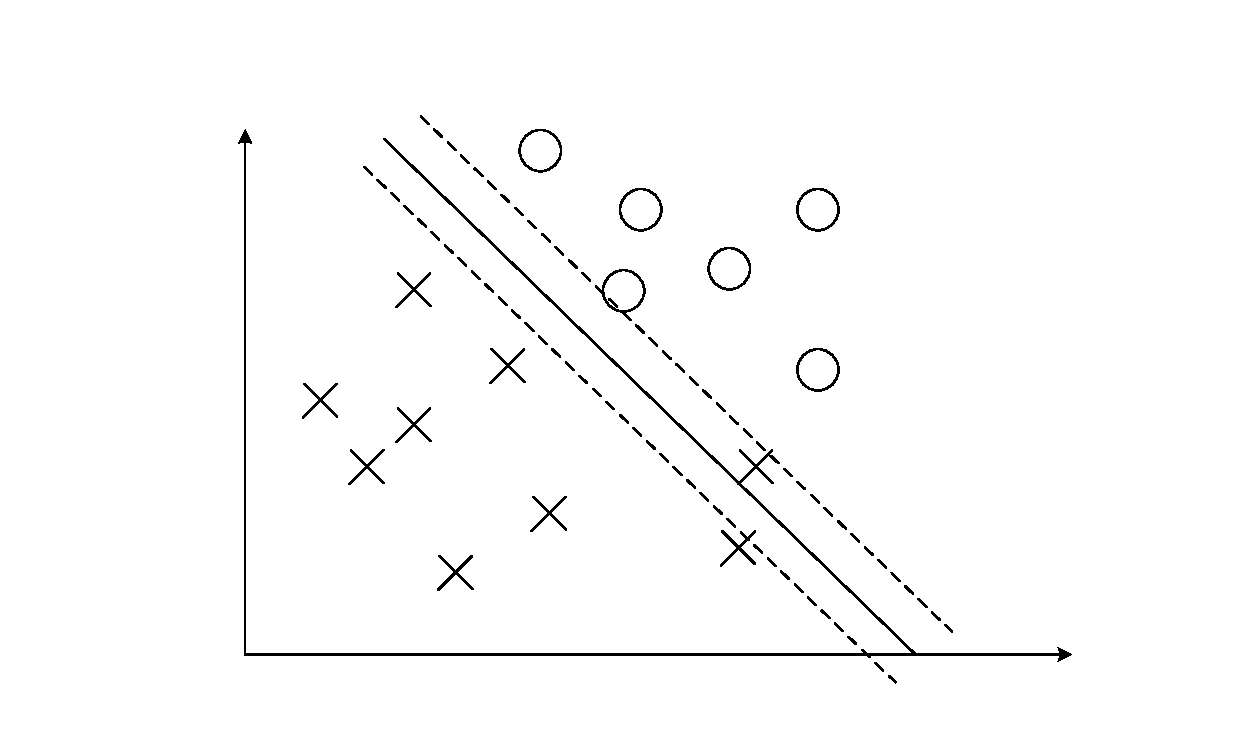
\includegraphics[width=\linewidth]{figures/SVM.pdf}
  \caption{Principle of SVM}
  \label{fig:SVM}
\end{figure}

I used the build-in \textit{SVM} module of \textit{sklearn}. The training step is realized by \textit{svm.SVC.fit}. After PCA, the data matrix reduced to a size of $50\times5896$, which can be read in to the memory in one time. Therefore, no batch method is needed to fit the model.

\subsection{Classify with Deep Learning Method}

The other required mission is to do the same classification with deeplearning method. The Neuron Network (NN) is actually a Multilayer Perceptron (MLP) with four layers (three hidden layers and one output layer). The structure of each layer is shown in Fig. \ref{fig:MLP}. Each neuron of layer $i$ is a linear combinations of the layer $i-1$'s activations. Then activative function is applied to the linear combination. For layer $i$, the transmission function is:
\begin{equation}
  a_{i,j} = \mathrm{act} \left(\sum_{j=0}^n {W_{i,j} \cdot a_{i-1, j} + b_i}\right)
\end{equation}
$a_{i, j}$ is the $j$th neuron of layer $i$, $W_{i, j}$ and $b_i$ is the parameter to be trained. $\mathrm{act}$ is active function, where I used ReLU function:
\begin{equation}
  \mathrm{act}\left(x\right)=\max \left(x, 0\right)
\end{equation}
In the output layer, the neuron number is equal to the number of catagory, which is 10 (Table \ref{tab:category}). To get the loss of the output, softmax function is applied first, which is:
\begin{equation}
  \sigma\left(x\right)_j = \dfrac{e^{x_j}}{\sum_{i=0}^n {e^{x_i}}}
\end{equation}
then cross entrophy is applied to the output of softmax function, which is:
\begin{equation}
  C = - \left[y\ln a + \left(1-y\right)\ln\left(1-a\right)\right]
\end{equation}
where $y$ is the label of dataset, $a$ is output of softmax function. The softmax function and cross entrophy function is realized through tensorflow build-in function \textit{tf.nn.softmax\_ cross\_ entropy\_ with\_ logits()} \cite{tensorflow.org}. The reason of utlizing build-in function instead of realize it with the equation is that the build-in function can avoid the gradient ovreflow brought by the large number of weights ( $22283\times200$ in the first input layer).

To train a good classifier with the method, I tried different learning rate, different initialization configuration and different regulization decay. Then I found the best parametes which is shown in Table \ref{tab:NNParameter}. Adam Optimizer is utilized. To converge faster, the initial learning rate is set as $1e-3$. L2 regularization is applied for the first hidden layer and L1 regularizaion is applied for other layers. Decay of regulazation is set as 1, which can better classify and maintain the balance between the training set and test set. After totally 500 iterations, a trained NN is achieved.

Because the number of sample I used is much smaller than the sample in the file. Moreover, in order to read each batch, the file is read from the first line to the last line, which cost much time. It is fatal because totally 1000 times the file is read during training. So before the training, the used batches is extracted and saved in \textit{train\_data.txt} and \textit{test\_data.txt} files. In these files, instead of representing each sample with a column, each sample is represented by a row with more than 20000 columns. Therefore, to read a batch, a continuous 100 line reading is enough. The reading time is much decreased.


\begin{figure}
  \centering
  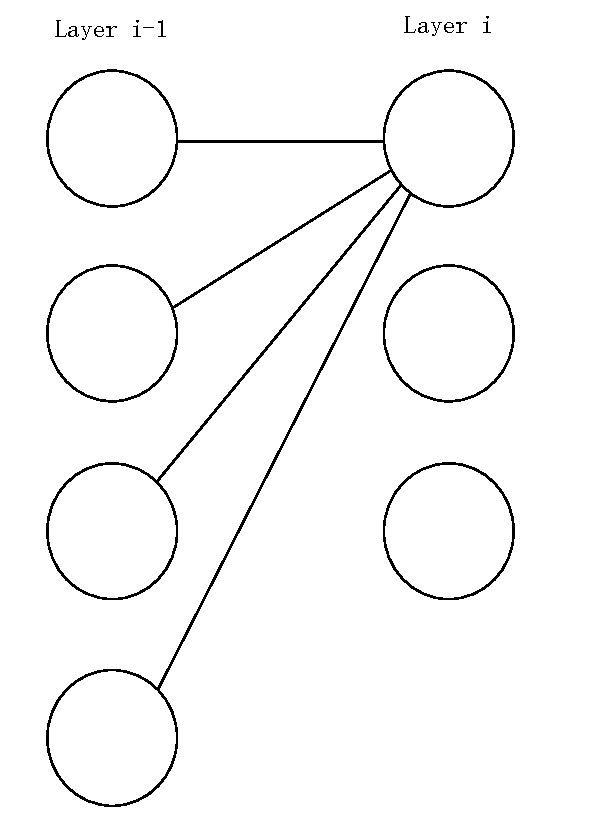
\includegraphics[width=0.5\linewidth]{figures/MLP.pdf}
  \caption{Structure of NN layer}
  \label{fig:MLP}
\end{figure}

\begin{table}
  \caption{NN Parameters, also the best configuration I found after many attemps}
  \label{tab:NNParameter}
  \begin{tabular}{cc}
    \toprule
    Parameter & Value \\
    \midrule
    Layer & 4 \\
    Neuron Number & 200, 50, 20 \\
    Active Function & ReLU \\
    Loss Function & Cross Entrophy\\
    Optimizer & Adam \\
    Batch Size & 100 \\
    Initial Learning Rate & $1e-3$ \\
    Regularization & L2 for layer1; L1 others \\
    Regularization Decay & 1 \\
    Iteration & 500 \\
    \bottomrule
  \end{tabular}
\end{table}

\section{Result}
\subsection{Result of PCA + SVM}
\subsubsection{Result of PCA}
After PCA, the deminsion of data is lowered to 50. Eigenvalue of the 50 factors is shown in Fig. \ref{fig:eigenvalue}. Most of the eigenvalues is smaller than 5, Only about 20 eigenvalues are larger than 5.

\begin{figure}[h]
  \centering
  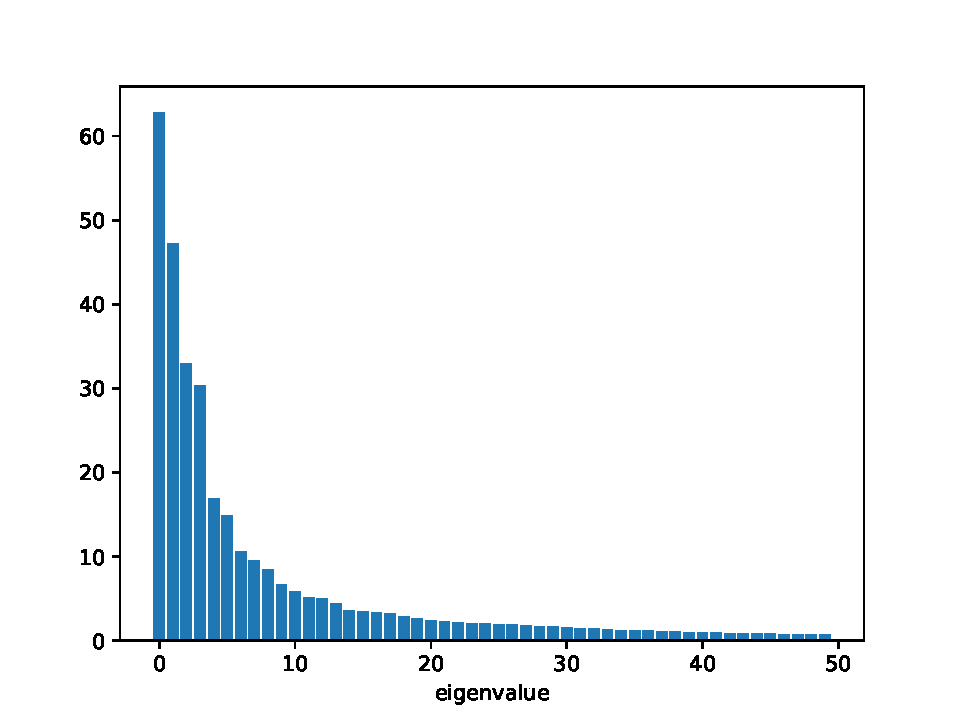
\includegraphics[width=\linewidth]{figures/eigenvalue.pdf}
  \caption{Eigenvalue of the 50 diminsion}
  \label{fig:eigenvalue}
\end{figure}

\subsubsection{Result of SVM Classification}

When all the 50 eigenvalues are used, the overall accuracy and accuracy of each catagories is shown in Table \ref{tab:AccuracySVM50}. Both the training set and the test set have achieved a high accuracy. The accuracy of training set (97.3\%) is a little higher than the testing set (94.6\%). This mean that the classification is a little overfitting. Looking at each individual catagory, the largest catagories, Leukemia (550 samples for training, 205 samples for test), Breast Disease (596 samples for training and 260 for test) and Brain Disease (288 samples for training and 129 samples for test), their train accuracy are over 99\% , with test accuracy no lower than 95\%. For small catagories, such as Bladder Disease (30 samples for training and 10 samples for test) and Normal (91 samples for training and 31 samples for test), their test accuracy are low (no more than 70\%), even if the training accuracy of Bladder Disease is higher than 90\%.

\begin{table}
  \caption{Accuracy of PCA + SVM, deminsion = 50}
  \label{tab:AccuracySVM50}
  \begin{tabular}{ccccc}
    \toprule
    Catagory & \multicolumn{2}{c}{Train} & \multicolumn{2}{c}{Test}\\
    & Number & Accuracy & Number & Accuracy\\
    \midrule
    Normal & 91 & 81.3\% & 31 & 45.2\% \\
    Leukemia & 550 & 99.2\% & 205 & 95.1\% \\
    Atopic & 43 & 95.3\% & 21 & 85.7\% \\
    B-cell & 155 & 99.3\% & 66 & 94.0\% \\
    Breast Disease &  596 & 99.5\% & 260 & 97.7\% \\
    Brain Disease & 288 & 99.3\% & 129 & 96.1\% \\
    Bone Disease & 108 & 96.3\% & 42 & 85.7\% \\
    Lung Disease & 50 & 96.0\% & 27 & 81.5\% \\
    Bladder Disease & 30 & 96.7\% & 10 & 60.0\% \\
    Intestinal Disease & 117 & 99.1\% & 36 & 94.4\% \\
    \midrule
    Totally & 2028 & 97.3\% & 827 & 94.6\% \\
    \bottomrule
  \end{tabular}
\end{table}

Varing the diminsion of training data, the accuracy of the SVM classifier is shown in Fig. \ref{fig:accuracy}. As we can see in Fig. \ref{fig:eigenvalue}, only 20 of the eigenvalues are larger than 5. So when varing the number of  diminsion from 50 to 20, the accuracy of training set does not fall, and is still 97.3\%. But meanwhile, the accuracy of test set fall from 94.6\% to 89.9\%. This means that the small diminsions is still important for the generalization of classifier. When deminsion reduces to 10, which means that some large deminsion is omitted, the accuracy of training set start to fall to 96.5\%.

\begin{figure}[h]
  \centering
  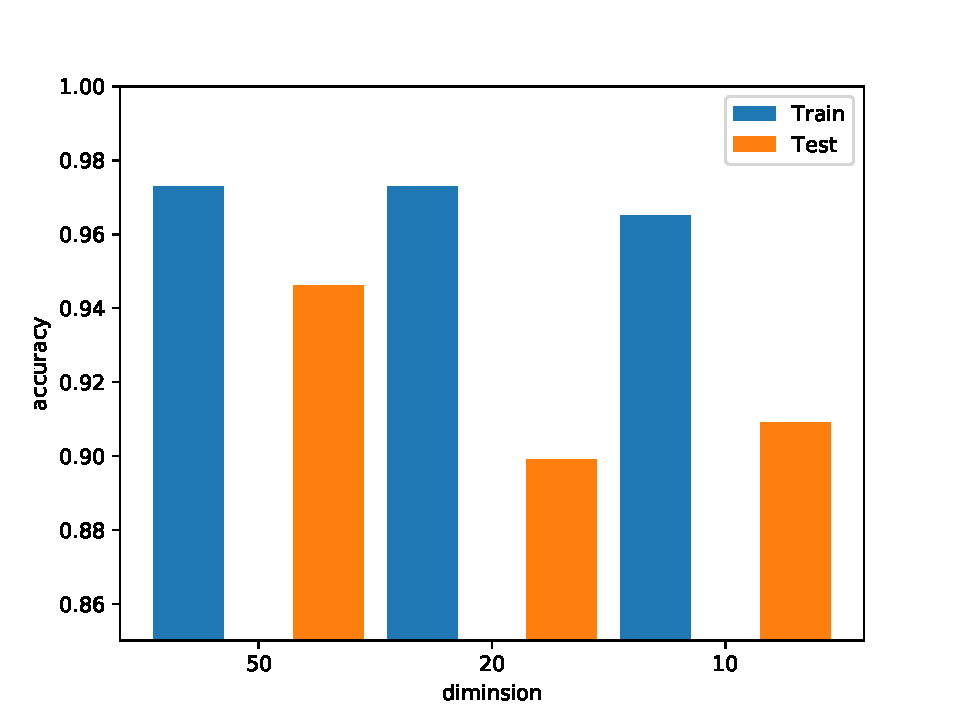
\includegraphics[width=\linewidth]{figures/accuracy.pdf}
  \caption{Accuracy varing the diminsion}
  \label{fig:accuracy}
\end{figure}
\subsection{Result of Deep Learning}

With the parameters in Table \ref{tab:NNParameter}, I trained the neuron network classifier. During the 100 iterations, the loss decreased and the accuracy increased. The change of loss and accuracy is shown in Fig. \ref{fig:loss_nn} and Fig. \ref{fig:accuracy_nn}. Both the accuracy of training set and test set increases during the training and stable at about 70\%.

\begin{figure}
  \centering
  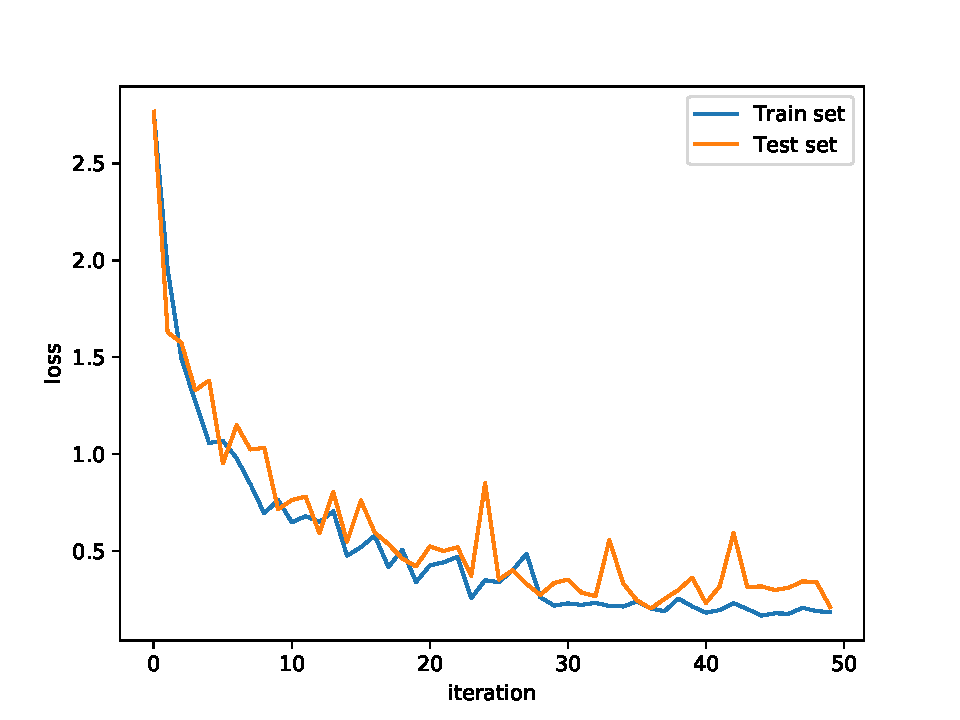
\includegraphics[width=\linewidth]{figures/loss_nn.pdf}
  \caption{Loss of trainning set and test set changing during training}
  \label{fig:loss_nn}
\end{figure}

\begin{figure}
  \centering
  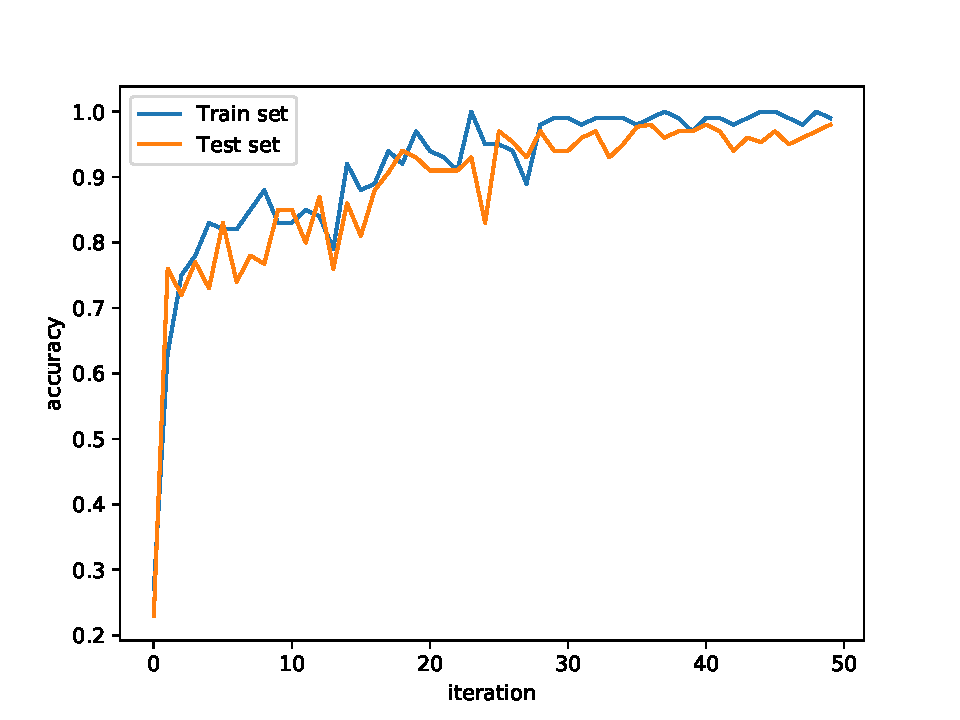
\includegraphics[width=\linewidth]{figures/accuracy_nn.pdf}
  \caption{Accuracy of trainning set and test set changing during training}
  \label{fig:accuracy_nn}
\end{figure}

The result of each categories is shown in Table \ref{tab:AccuracyNN}. It can be seen that for small categories, such as Bladder Disease
(30 samples for training and 10 samples for test), both the training accuracy and test accuracy is larger than 95.0\%. And for large categories, such as B-cell (155 samples for training and 66 samples for test), Breast Disease (596 samples for training and 260 samples for test), both the training set accuracy and test set accuracy is high, which is almost 100\%. All the accuracies are higher than using traditional SVM and PCA method.
\begin{table}
  \caption{Accuracy of NN, number of neuron (200, 50, 20)}
  \label{tab:AccuracyNN}
  \begin{tabular}{ccccc}
    \toprule
    Catagory & \multicolumn{2}{c}{Train} & \multicolumn{2}{c}{Test}\\
    & Number & Accuracy & Number & Accuracy\\
    \midrule
    Normal & 91 & 96.3\% & 31 & 66.7\% \\
    Leukemia & 550 & 99.8\% & 205 & 98.6\% \\
    Atopic & 43 & 100.0\% & 21 & 100.0\% \\
    B-cell & 155 & 99.4\% & 66 & 100.0\% \\
    Breast Disease &  596 & 99.7\% & 260 & 99.5\% \\
    Brain Disease & 288 & 100.0\% & 129 & 99.3\% \\
    Bone Disease & 108 & 100.0\% & 42 & 100.0\% \\
    Lung Disease & 50 & 100.0\% & 27 & 93.1\% \\
    Bladder Disease & 30 & 96.6\% & 10 & 100.0\% \\
    Intestinal Disease & 117 & 100.0\% & 36 & 100.0\% \\
    \midrule
    Totally & 2028 & 100.0\% & 827 & 99.0\% \\
    \bottomrule
  \end{tabular}
\end{table}

To research how the number of neuron influence the result, I varied the number of neuron of the first hidden layer. I varied the number by and the result is shown in Table \ref{tab:varingneuron}. It can be seen that with fewer neurons, the accuracy of the network has a little decrease. But the decrease is not much. In Table \ref{tab:AccuracyNN_small}, I present the accuracy of each categories with fewer neurons. We can find that difference between the accuracy of each categories increased.

\begin{table}
  \caption{Result of NN Varing the number of neuron}
  \label{tab:varingneuron}
  \begin{tabular}{ccc}
    \toprule
    \#Neuron & Training Accuracy & Test Accuracy \\
    \midrule
    (200, 50, 20) & 100.0\% & 99.0\% \\
    (100, 50, 20) & 97.0\% & 95.0\% \\
    (50, 30, 20) & 99.0\% & 97.0\% \\
    (30, 20, 15) & 99.0\% & 95\%\\
    \bottomrule
  \end{tabular}
\end{table}

\begin{table}
  \caption{Accuracy of NN, number of neuron (50, 30, 20)}
  \label{tab:AccuracyNN_small}
  \begin{tabular}{ccccc}
    \toprule
    Catagory & \multicolumn{2}{c}{Train} & \multicolumn{2}{c}{Test}\\
    & Number & Accuracy & Number & Accuracy\\
    \midrule
    Normal & 91 & 78.8\% & 31 & 57.1\% \\
    Leukemia & 550 & 99.6\% & 205 & 98.6\% \\
    Atopic & 43 & 97.7\% & 21 & 100.0\% \\
    B-cell & 155 & 98.8\% & 66 & 100.0\% \\
    Breast Disease &  596 & 99.8\% & 260 & 100.0\% \\
    Brain Disease & 288 & 100.0\% & 129 & 99.3\% \\
    Bone Disease & 108 & 93.3\% & 42 & 97.8\% \\
    Lung Disease & 50 & 100.0\% & 27 & 82.8\% \\
    Bladder Disease & 30 & 72.4\% & 10 & 63.6\% \\
    Intestinal Disease & 117 & 100.0\% & 36 & 100.0\% \\
    \midrule
    Totally & 2028 & 99.0\% & 827 & 97.0\% \\
    \bottomrule
  \end{tabular}
\end{table}

\section{Discuession}

From the result, both the traditional PCA + SVM method and deep learning method can classify the samples well. But for small categories, SVM + PCA is not better than deep learning method. Neuron network performs better for classifying small categories. With fewer parameters, both the two method performs worse. Even if the total accuracy does not fall too much for neuron network, the accuracy of small categories still fall evidently.

%%
%% The acknowledgments section is defined using the "acks" environment
%% (and NOT an unnumbered section). This ensures the proper
%% identification of the section in the article metadata, and the
%% consistent spelling of the heading.
\begin{acks}
Thanks for instructor of this class Prof. Bo Yuan and assistants of the class. They gave me the chance to research the project.
\end{acks}

%%
%% The next two lines define the bibliography style to be used, and
%% the bibliography file.
\bibliographystyle{ACM-Reference-Format}
\bibliography{sample-base}
.

\end{document}
\endinput
%%
%% End of file `sample-sigchi.tex'.
